\subsection{Ejercicio 3: Comparación de Escenarios de Demanda Final}

En este ejercicio se compararon tres escenarios de demanda final: conservador (-10\%), base (demanda actual) y optimista (+15\%), calculando la producción requerida para cada uno.

\subsubsection{Demanda Final por Escenario}

\begin{table}[H]
\centering
\caption{Demanda Final por Escenario}
\begin{tabular}{lccc}
\toprule
Sector & Conservador (-10\%) & Base & Optimista (+15\%) \\
\midrule
Agricultura & 2.70 & 3.00 & 3.45 \\
Tecnología & 3.60 & 4.00 & 4.60 \\
Servicios & 7.20 & 8.00 & 9.20 \\
\bottomrule
\end{tabular}
\end{table}

\subsubsection{Producción Total Requerida por Escenario}

\begin{table}[H]
\centering
\caption{Producción Total Requerida por Escenario}
\begin{tabular}{lccc}
\toprule
Sector & Conservador & Base & Optimista \\
\midrule
Agricultura & 4.32 & 4.80 & 5.52 \\
Tecnología & 7.09 & 7.88 & 9.06 \\
Servicios & 10.53 & 11.70 & 13.46 \\
\bottomrule
\end{tabular}
\end{table}

Los resultados muestran que el escenario conservador reduce la producción requerida en un 10.0\% para Agricultura, 10.0\% para Tecnología y 10.0\% para Servicios. El escenario optimista aumenta la producción requerida en un 15.0\% para Agricultura, 15.0\% para Tecnología y 15.0\% para Servicios. Esto demuestra la sensibilidad de la economía a los cambios en la demanda final.

\begin{figure}[H]
\centering
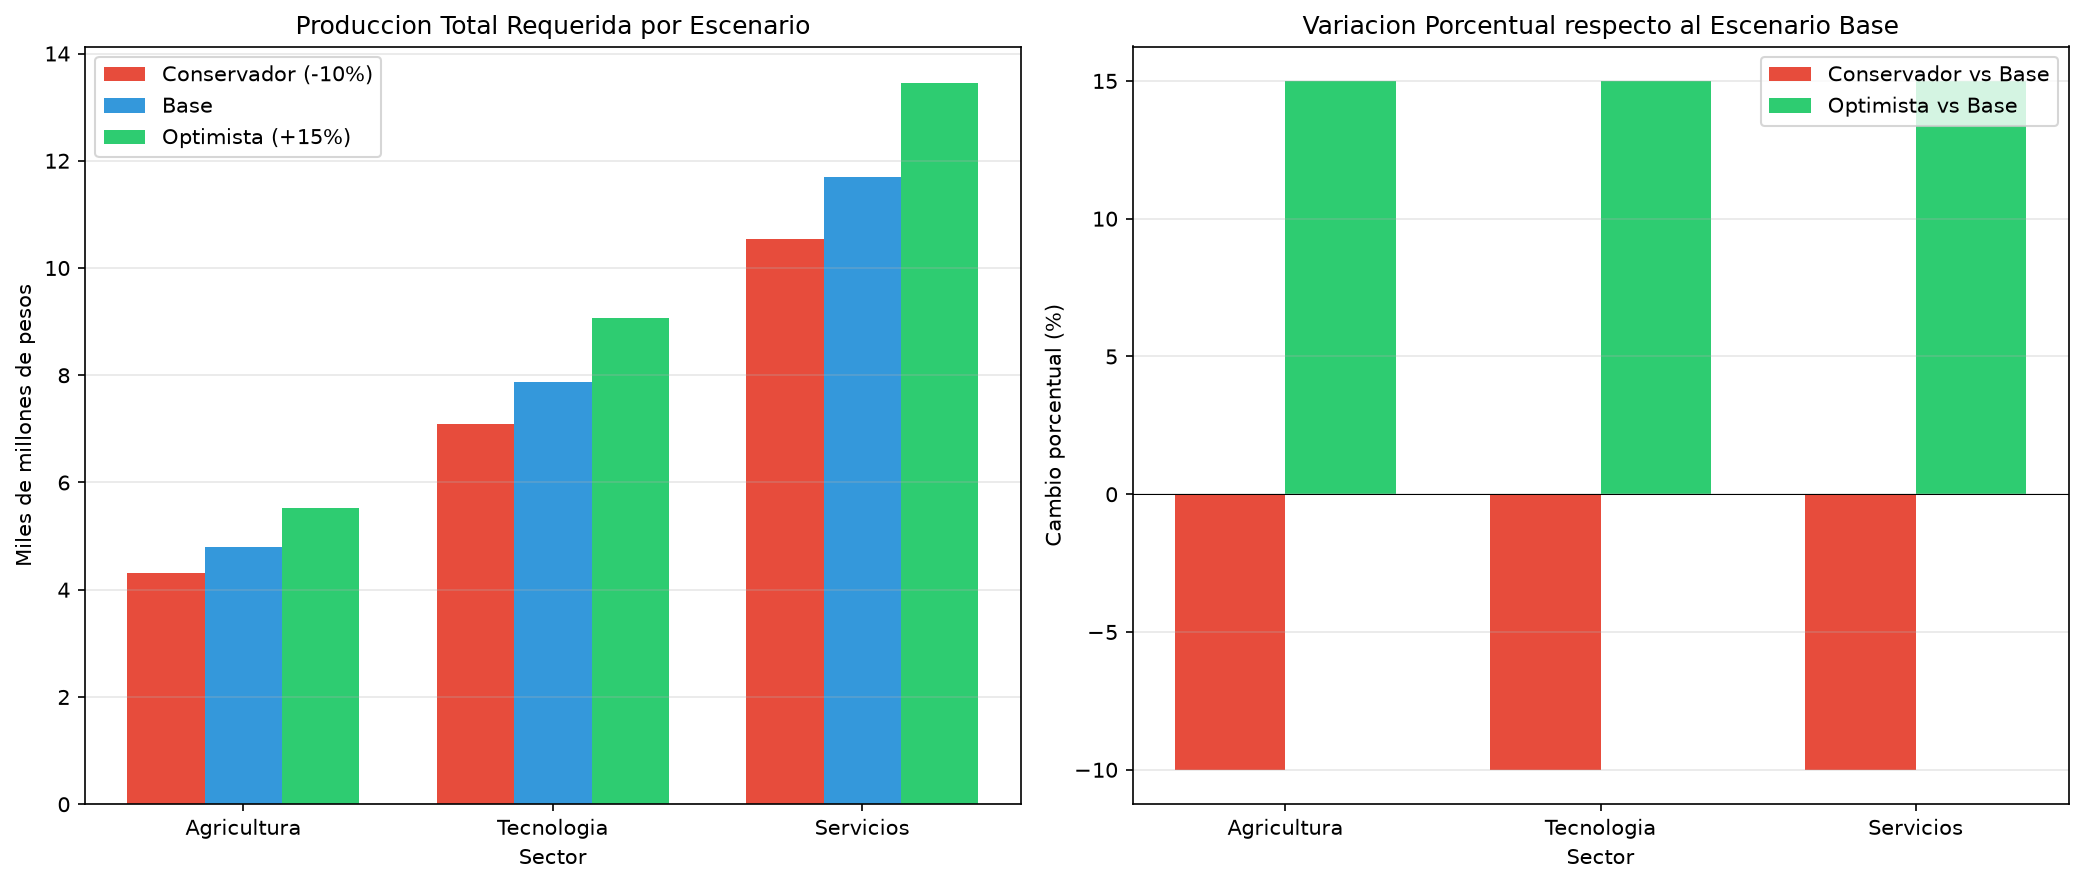
\includegraphics[width=0.9\textwidth]{ejercicio3_escenarios/resultados_escenarios.png}
\caption{Comparación de Escenarios de Demanda Final}
\end{figure}

\clearpage
